\section{Motivation and Propane overview}
\label{sec:motivation}

%We motivate our work by describing the current practice in network
%configuration. In traditional networks with distributed control planes, the operators' goal is to generate the configuration of individual devices based on their desired policy. This configuration dictates the behavior of a device, how it exchanges routing information with neighbors and how it filters and ranks that information. The collective behavior of the devices should implement the desired policy.
%
%Device configuration languages are low-level and indirect. For instance, instead of allowing operators to express directly the paths they want through the network, they require operators to specify metrics that result in those paths; instead of allowing operators to express directly the types of traffic to not carry through the network, they require operators to select and program an appropriate filtering mechanism (e.g., BGP import or export filters, null routing,  access control lists) and instantiate it on topologically appropriate devices; instead of allowing operators to directly specify that they prefer BGP neighbors in a certain order, they require operators to program local preferences and multi-exit discriminators (MED) at each router and ensure that the numbers are consistent across routers.
%
%In many networks today, device configurations are generated manually by operators, without the support of many automated tools. It is easy to see the problems with this approach, such as typos, inconsistency across devices, and no guarantees of policy compliance.
%
%To reduce such problems, some networks use a template-based approach. Configuration templates abstract certain constants into variables (e.g., instead of concrete community value, they may contain a variable {\small \sf{\$$BadNeighbor$)}} and may use a device vendor-neutral syntax. Operators manually generate the templates and use tools to translate them into device configuration, by replacing variables with appropriate constants using a database of network information.
%
% %and replacing vendor-neutral constructs with their vendor-specific counterparts.
%
%%In practice, most networks use a hybrid of templates and manual generation of device configuration. Templates are used for standardized and common configuration elements across devices and the result is manually tweaked to obtain the exact desired network behavior.
%
%While templates avoids some pitfalls of the fully manual approach, they too are far from ideal. The fundamental issue is the semantic mismatch between desired policies and the level of abstraction of templates. While many policies are network-wide (e.g., prefer customer networks, or never announce a route to a certain prefix to external neighbors), templates are device-level. Operators must still manually decompose network-wide policies into device-level policies that can produce the desired network-wide behavior.
%This decomposition is not always straightforward and ensuring policy-compliance can be hard, especially in the face of failures. We illustrate this point using two examples based on policies that we have seen in practice and we demonstrate the ease with which the
%examples are described using our new language \sysname.

In networks with distributed control planes, the operators today generate the configuration of individual devices based on intended policy. Whether this task is done fully manually or with the aid of templates, the challenge is to decompose network-wide policies
%(e.g., prefer customer networks, or never announce a route to a certain prefix to external neighbors),
into device-level policies that collectively produce the intended behavior.
This decomposition is not always straightforward and ensuring policy-compliance can be hard, especially in the face of failures. We illustrate this point using two examples based on policies that we have seen in practice. We also demonstrate the ease with which the
policies can be specified using our new language \sysname. The next section describes how to automatically compile this specification to device-level policies.

\begin{figure}[t!]
\centering
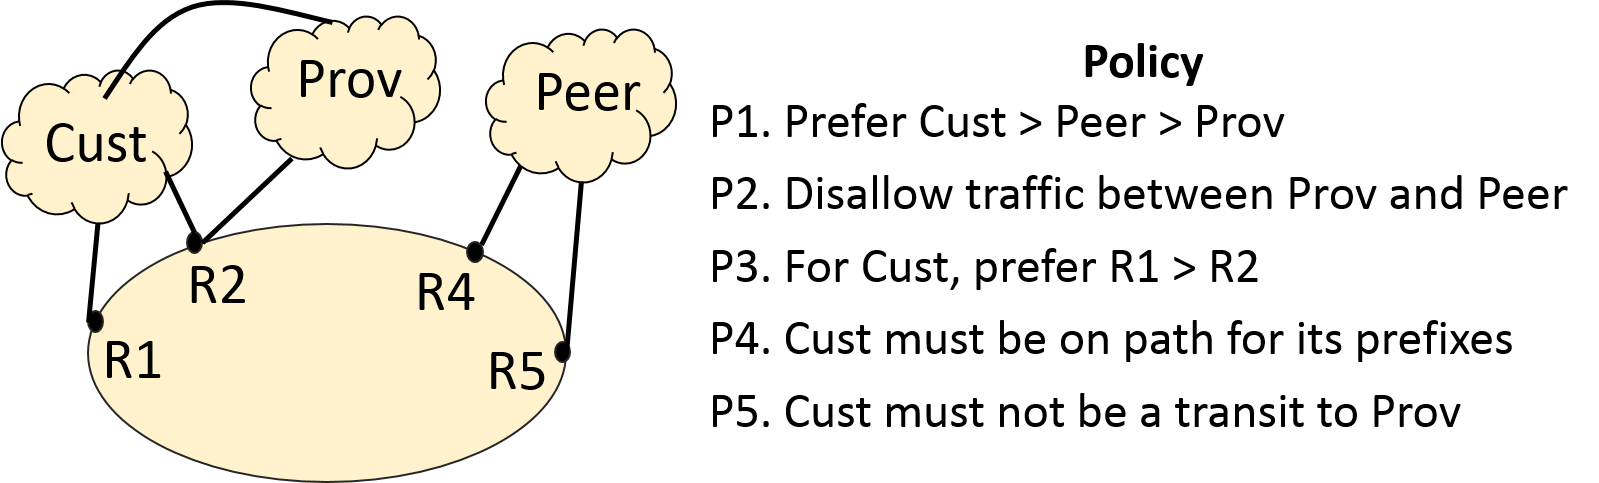
\includegraphics[width=\columnwidth]{figures/example1}
\caption{Creating router-level policies is difficult.}
\label{fig:example1}
\end{figure}

\subsection{Example 1:  The Backbone}

Consider the backbone network in Figure~\ref{fig:example1}. It has three neighbors, a customer $Cust$ , a peer $Peer$, and a provider $Prov$. The policy of this network is shown on the right. It prefers the neighbors in a certain order ($P1$) and does not want to act as a transit between Peer and Prov ($P2$). It prefers to exchange traffic with Cust over $R1$ rather than $R2$ because $R1$ is a cheaper ($P3$). To guard against another AS "hijacking" prefixes owned by Cust, it only sends traffic to them if Cust is on the AS path ($P4$). Finally, to guard against Cust accidentally becoming a transit for Prov, it does not use Cust for traffic that will later traverse Prov ($P5$).

To correctly implement this policy, the operators must compute and assign local preferences such that preferences at Cust-facing interfaces $>$ Peer-facing interfaces $>$ Prov-facing interfaces. At the same time, the preference at $R2$'s Cust-facing interface should be lower than that at $R1$, but higher than that at Prov-facing interface. To fully realize $P2$, MEDs will have to be appropriately configured as well. To implement $P3$ and $P4$, the operators may assign communities that indicate where a certain routing announcement entered the network. Then, R4 must not announce to $Peer$ routes that have communities that correspond to the R2-prov link but must announce communities for the $R2$-Cust and $R1$-Cust links. Finally, to implement $P4$ and $P5$, the operators will have to compute and configure appropriate prefix- and AS-path-based filters at each router.

We can now see how devising correct configuration for real, larger networks will quickly become a nightmare. The networks will have many neighbors across multiple classes of commercial relationships, differing numbers of links per neighbor, along with several region-, neighbor- or prefix-based exceptions to the default behavior. Templates help by keeping preference and community values consistent across routers, but operators must still do much of the conceptually difficult work manually.
%, in coming up with the templates themselves.

\begin{figure}[t!]
\centering
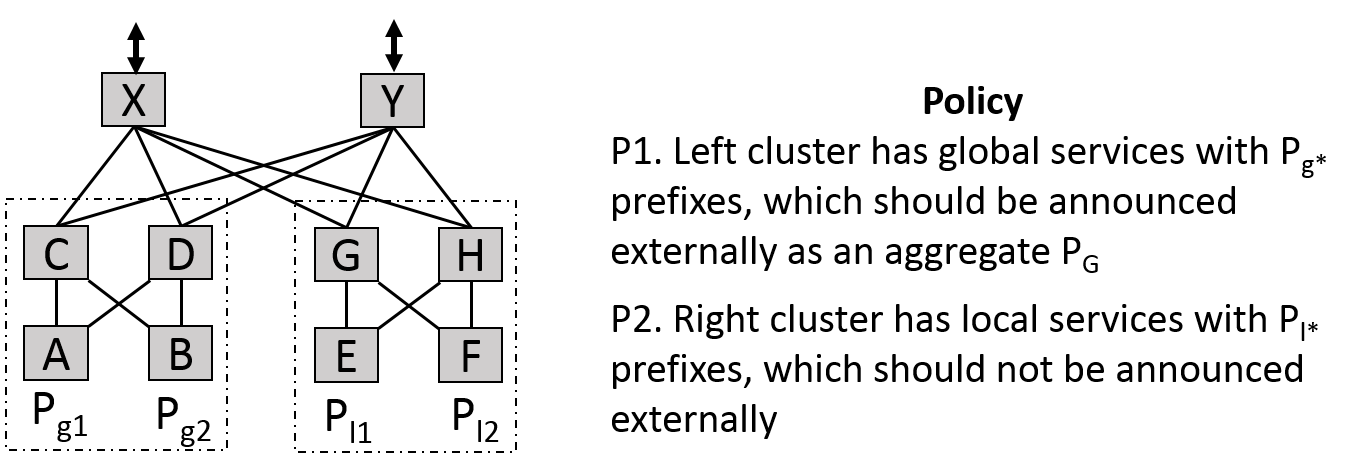
\includegraphics[width=\columnwidth]{figures/example2}
\caption{Policy-compliance under failures is difficult.}
\label{fig:example2}
\end{figure}

\para{The Backbone in \sysname}
\sysname simplifies network configuration by allowing users to
specify end-to-end forwarding paths and associating them with
appropriate prefixes.  The \sysname compiler handles the task of
generating low-level BGP configurations consistent with the user's
specifications.  It automatically synthesizes
import-export filters, local preferences, MED attributes, and community tags
to ensure policy compliance under all possible failure scenarios.

In general, \sysname specifications are written modularly via a series
of user declarations.
%These definitions allow users to express the three
%major elements of any \sysname specification:  \emph{prefixes},
%\emph{paths} and \emph{policies}.
For example, to begin specification of the backbone
network, we first express the idea that for routes leading to our customer,
we prefer using $R_1$ over $R_2$ (Policy P3 from Figure~\ref{fig:example1}):
\begin{lstlisting}[mathescape=true]
define ExitCust = $exit(R_1 \gg R_2)$
\end{lstlisting}
The  statement above defines a set of \emph{ranked paths}, which includes
all paths (and only those paths) that \cd{exit}
our network
through either router $R_1$ or $R_2$.  The paths that exit through $R_1$
are preferred ($\gg$) to the paths that exit through $R_2$.

To associate ranked paths with
one or more prefixes, we must define a \sysname \emph{policy}.
Within a policy, statements with the form $\path{x}{p}$
associate the prefixes defined by the predicate $x$ with the set of
ranked paths defined by the path expression $p$.
For instance, in the following code, ranked paths are associated with
the customer prefixes ($C_{pfx}$), the internal prefixes ($I_{pfx}$),
and all other prefixes (\cd{true}).\footnote{Policy statements are processed in
order with earlier policy statements taking precedence over later
policy statements.  Hence, when the prefix predicate \cd{true} follows
statements involving $C_{pfx}$ and $I_{pfx}$, it is interpreted as
$\cd{true} \AND \NOT C_{pfx} \AND \NOT I_{pfx}$.}

\begin{lstlisting}[mathescape=true]
define Routing = {
    $\path{C_{pfx}}{ExitCust \gg end(Cust)}$
    $\path{I_{pfx}}{end(in)}$
    $\path{true}{ExitCust \gg exit(Peer) \gg exit(Prov)}$
}
\end{lstlisting}

Line 2 of the policy above
defines the paths that exit our network to customer prefixes ---
\cd{ExitCust} defines paths through $R_1$ and $R_2$ and in the event
that connections to the customer through both of those routers fail,
a backup route ($end(Cust)$) is defined that admits traffic to go through
any path that ends at the customer.
Line 3 states that traffic for internal prefixes must end in our network, and is otherwise unconstrained.  The special keyword \cd{in} represents any location
inside the user's network whereas the keyword \cd{out} represents any location
outside the user's network.
Line 4 applies to any other traffic, and allows for any routes that leave through a peer with a preference for customers over peers over providers. To summarize our progress so far, the \cd{Routing} policy
implements (P1), (P3) and (P4) from Figure~\ref{fig:example1}

Since, routing still allows transit traffic (e.g., traffic can enter from \textit{Peer} and leave through \textit{Prov}), we can define a new policy that
implements this restriction separately.

\begin{lstlisting}[mathescape=true]
define PP = Peer or Prov
define PPTransit = $enter(PP) \AND exit(PP)$
define CustTransit = $later(Cust) \AND later(Prov)$

define NoTransit = {
    $\path{true}{\neg PPTransit \AND \NOT CustTransit}$
}
\end{lstlisting}

The \textsf{NoTransit} constraint above ensures that requirements (P2) and (P5) are satisfied. In particular, it says that for any prefix, traffic should never both enter and exit the network from \textit{Peer} or \textit{Prov}. Similarly it prevents traffic from ever following paths that leave our network and later passing through both \textit{Prov} and \textit{Cust}.  To implement both \cd{Routing}
and \cd{NoTransit} simultaneously, we simply conjoin them:

\begin{lstlisting}[mathescape=true]
Routing $\AND$  NoTransit
\end{lstlisting}

\sysname will generate per-device import and export filters, local preferences,
MED attributes, and community tags to ensure that the policy is
implemented correctly under all failure scenarios.

\subsection{Example 2:  The Data Center}

If configuring policies for a fully functional network is difficult, doing so in a way that ensures policy compliance in the face of failures can be almost impossible. Consider the data center network in Figure~\ref{fig:example2} with routers organized as a fat tree and running BGP.\footnote{To scale and to simplify policy implementation, data center networks increasingly use BGP internally, with a private AS number per router~\cite{bgp-in-dc-rfc}.} The network has two clusters, one that hosts services that should be reachable globally and one that hosts that should be accessible only internally. This policy is enabled by using non-overlapping address space in the two clusters and ensuring that only the address space for the global services is announced externally. In addition, to reduce the number of prefixes that are announced externally, the global space is aggregated into one larger, less-specific prefix $P_G$. The semantics of aggregation in BGP is that the aggregate prefix is announced as long as the router has a path to even one sub-prefix.

The operator may decide that a simple way to implement the policy is to have X and Y: $i)$ not export externally what they hear from routers G and H since these routers border the cluster with local services; and $ii)$ announce what they hear from routers C and D and aggregate to $P_G$ if an announcement is subset of $P_G$. The appeal of this implementation is that X and Y do not need to be made aware of which prefixes are global versus local and IP address assignment can be done independently (e.g., new prefixes can be added to local services without updating router configurations).

However, this implementation is incorrect because it does not have the right behavior in the face of failures. Suppose links X--G and X--H fail. Then, X will hear announcements for $P_{l*}$ from C and D, having traversed from G and H to Y to C and D. Per policy implementation, X will start "leaking" these prefixes externally. Depending on the rationale for local services, this leak could impact security (e.g., if the services were sensitive) or availability (e.g., if the $P_{l*}$ prefixes are used for other services outside of the data center). This problem does not manifest without failures because then X has and prefers paths to $P_{l*}$ through G and H since they are shorter. A similar problem will happen if links Y--G and Y--H fail.
%\footnote{A different problem occurs when links X--C and X--D (or Y--C and Y--D) fail. X (Y) may stop announcing the global prefixes because they would be heard through G and H.}
Link failures in data centers are frequent and it is not uncommon to have multiple failed links at a given time~\cite{dc-failure-study}.

To avoid this problem, the operator may decide to disallow paths with "valleys," i.e., those that go up, down, and back up again. This safeguard can be implemented by $X$ and $Y$ rejecting paths through the other. However, that creates a different problem in the face of failures---an aggregation-induced blackhole~\cite{xx}. Suppose links D--A and X--C fail. Now, X will hear announcements for $P_{g2}$ from D and will thus announce the $P_G$ externally. This announcement will bring to X traffic for $P_{g1}$ as well, but because of valley-free filtering, X does not have a valid route for $P_{g1}$ and will thus drop all traffic to it.

Thus, we see that devising a configuration that ensures policy compliance in the face of failures is complex and error-prone. \sysname helps operators by implementing their high-level policy specification in a way that guarantees compliance under all failures if that is possible. Otherwise, it generates a compile-time error that informs them that the specification cannot be met. For aggregation, it will also provide a lower bound to operators on the number of failures under which aggregation will not result in blackholes.

\para{The Data Center in \sysname}
In our data center example,
there are primarily three main concerns:
(1) traffic for the prefix block allocated to each top-of-rack router must be able to reach that router,
(2) local services must not leak outside the datacenter, and
(3) aggregation must be performed on global prefixes to reduce churn
in the network.

\sysname allows us to decompose and specify each of these constraints in a modular fashion. The first constraint is about prefix ownership -- namely, that we only want traffic for certain prefixes to end up at a particular locations. The following definition captures this intent.

\begin{lstlisting}[mathescape=true]
define Ownership = {
    $\path{p_{g1}}{end(A)}$
    $\path{p_{g2}}{end(B)}$
    $\path{p_{l1}}{end(E)}$
    $\path{p_{l2}}{end(F)}$
}
\end{lstlisting}

In English: traffic for prefix $p_{g1}$ is only allowed to follow paths that
end at router A; traffic not matching $p_{g1}$, but which matches $p_{g2}$ must
end at router B; and so on.

To capture the second constraint, we can define another task for the core
routing policy:

\begin{lstlisting}[mathescape=true]
define Routing = {
    $\path{p_{g*}}{any}$
    $\path{p_{l*}}{\NOT enter(out)}$
    $\path{true}{exit(out)}$
}
\end{lstlisting}

The first line states that there is no restriction (\cd{any})
on how traffic must
traverse the network for global prefixes, aside from the default restriction
that traffic must not pass through the user's network and then loop
back on itself. This means traffic for
$p_{g*}$ may be sent either from other routers in the datacenter, or
from external ASes. The second line ensures that traffic for local
prefixes never enters the network from an outside location. This constraint
guarantees that the services remain reachable only to locations
internal to the data center.

As in the backbone example, we can combine these constraints
logically to specify the network-wide policy.
However, in addition to constraints on the shape of paths,
\sysname allows the operator to specify constraints on the BGP control plane.
For instance, a constraint on aggregation is included to ensure that
aggregation for $p_{agg}$ is performed from locations inside the network
to locations outside the network. \todo{Say more about aggregation here.
What prefixes are aggregated in to what blocks?  How is this defined?}

\begin{lstlisting}[mathescape=true]
Ownership $\wedge$ Routing $\wedge$ agg($p_{agg}$, $in \rightarrow out$)
\end{lstlisting}

As before, once \sysname compiles the policy, it is guaranteed to hold under
all possible failure scenarios. In addition, the system can check for
aggregate-induced black holes in the presence of up to $k$ failures.
\todo{Note:  Another comment about failure checking for black holes, which may
not be implemented yet.}


%\subsection{OLD -- Overview}
%\todo{this subsection can be deleted once we have captured everything in it}
%
%Sources of bugs we fix. (It seems like the main advantage of our approach is not just fixing bugs though - it is easily describing high-level intention).
%Perhaps the best way to do this is by going through a bunch of examples in section 2 and showing how you could easily introduce bugs:
%
%\begin{itemize}
%	\item Out of sync, or copy paste errors due to replicated configs (never an issue due to centralized control)
%	\item Correct filtering to ensure no undesired traffic can flow through the network (e.g., best practices, like an AS should filter customers for their prefix, are implemented automatically )
%	\item Failures can easily lead to unexpected behavior (e.g., a datacenter failure scenario w/instability.)
%	\item Trying to do anything interesting, like get backups correct is difficult (e.g., setting up aggregation wrong)
%	\item Related to the last point, things like aggregation can introduce black holes. We have the information needed to prevent this
%\end{itemize}
%
%
%Possible Examples:
%\begin{itemize}
%	\item Basic datacenter with spine preference
%	\item Simple AS that prefers customers over peers over providers
%	\item Combined internal backup routing with preference based entrance into the network using aggregation.
%	\item Something like cold potato routing
%\end{itemize}

